\documentclass{jarticle}

\usepackage{geometry}
\usepackage{cite}
\usepackage[dvipdfmx]{graphicx}
\usepackage{here}
\usepackage{amsmath}
\usepackage{amsfonts}
\bibliographystyle{junsrt} %参考文献出力スタイル


\geometry{left = 20mm, right = 20mm}
\title{ホモロジーの永続性を利用した異常検知}
\author{黒木 裕鷹}
\date{2018年4月27日}

\begin{document}
\maketitle
\section{はじめに}
現在,世界の様々な工場では産業用ロボットが用いられている.そのような工場では,重量物の運搬を必要としたり,霧散している粉塵を吸い込んだりする危険性など,人間には負担の大きい作業の割合が多い.
産業用ロボットはこのような安全性の問題を解決するだけでなく,経済性や効率性においてもメリットがある.
しかし同時にロボットには故障のリスクがあり,ただひとつのロボットの故障が生産ライン全体に影響を及ぼし得る.
故障を未然に回避するためにはメンテナンスなどの保守作業を行うことが重要であるが,メンテナンスや部品交換にも費用や時間などコストがかかるため,適切なタイミングで行われることが望ましい.


自動車メーカーのMでは,生産ラインで使用するアームロボットの故障を未然に防ぐため,その減速機の交換を経験に基づくタイミングで行っている.
交換のタイミングが遅すぎれば故障を招くが,早すぎても交換に時間がかかる分パフォーマンスが低下することとなる.
本調査では,ロボットアームをモニタリングした振動のセンサーデータを用い,減速機交換前後のデータに明確な違いがあるかどうかを調査した.
ロボットの故障により生産ラインを止めることはあってはならないため,故障直前のデータは得ることが出来ないことに留意しなければならず,教師無し学習によるクラスタリングを行うことを目的とした.


Mより提供されたデータは一つのロボットアームにつき,減速機交換前後それぞれで5秒間の計測を10回行った1次元の振動データである.
ロボットアームはそれぞれ挙動が異なるため,その主要な振動はアームごとに異なっている.
また,各アームの行動1セットは5秒間ではないため,各計測ごとにより行動セットの中の計測する部分が異なっている.

クラスタ分析では,クラスタリングされる対象間の類似度もしくは非類似度が必要である.
時系列を対象としたクラスタリングにおいて,最も広く使用されている尺度はユークリッド距離,Dynamic Time Warping(DTW),CORTなどである.
DTWは2つ時系列データの時刻を$t_1$, $t_2$とすると,$t_1,t_2$全ての組の誤差を計算し,それらの合計が最小になるような経路を求めるアルゴリズムである.
DTWにより挙動の計測開始時点が異なる問題は多少解決されるが,振動の主な挙動はアームによって異なるため,減速機交換前後の差異はクラスタリングの結果に表れない.
また,未知音源分離で用いられる独立成分分析(ICA)は主要な振動と微細な振動を分けることを可能にするかもしれないが,同時点の複数観測を必要とするため本データには適用することはできない.
つまり時系列の同時性を利用することなく,かつアームごとに異なる主要な振動に影響されない特徴量によって教師無し学習を行うことが課題である.


本調査では,以上のような課題を解決するため,データの位相的な特徴に注目した.
近年着目されているTopological Data Analysis(TDA)は複雑なデータを扱う上で強力であり,パーシステント・ホモロジーをはじめとするその手法はデータの位相的特徴を抽出し,新しい知見を与える.
またTDAの分野で広く行われているように,時間遅れ座標を用いて時系列を多次元に埋め込むことで位相的特徴を抽出する足掛かりとした.
時間遅れ座標による埋め込みはダイナミカルシステムの分野で,状態空間の復元を目的に広く用いられている.

本レポートの構成は次のようである.
まず2節では本調査で使用したTDAの手法やクラスタリング手法について述べ,3節では実際のデータ解析とその結果を示す.
4節では考察を行うと共に今後の展望について触れる.

\section{Topological Data Analysis(TDA) と時系列クラスタリング}
トポロジーを用いてデータの情報を抽出するものであり,その主要な手法はmapper\cite{Singh2007}とパーシステント・ホモロジー\cite{Edelsbrunner2002}である.
これらはノイズを含む複雑なデータセットから何か新たな知見を得る目的でしばしば用いられてきた.
本調査ではパーシステント・ホモロジーを利用する.

\subsection{パーシステント・ホモロジー}
距離空間$(M, d_M)$の有限点集合を$X$,$X$を中心とした半径$r$の級の和集合を$B(X;r):=\bigcup_{i=1}^n B(x_i;r)$とする.
ただし,$B(x;r) =\{y \in M | d_M(x,y) \leq r\}$とする.
級の和集合を半径パラメータ$r$で集めた集合$\mathbb B(X):=\{B(X;r)\}_{r\geq 0}$をここでは$X$のフィルトレーションという.
$r\leq a$ならば包含関係$B(X;r)\subset B(X;a)$があるため、ホモロジー群間の射$u_r^a : H_q(B(X;r))\rightarrow H_q(B(X;a)) $を包含写像から誘導する。
このとき、ホモロジー群の系列
$$
H_q(\mathbb B(X)):\dots\rightarrow H_q(B(X;r))\overset{u_a^b}{\rightarrow} H_q(B(X;a))\rightarrow\dots (r\leq a)
$$
を$X$の$q$次元パーシステントホモロジーという。
パーシステントホモロジー体係数多項式環や$A_n$型箙の表現などの言葉で解釈することが出来、分解定理により適切な区間表現$\mathbb I[b_i, d_i] $を通じて
$$
H_q(\mathbb B(X))\cong\oplus\mathbb I[b_i,d_i] (b_i\leq d_i)
$$
と分解される。これをユークリッド空間$\mathbf R^2$内に表示した多重集合
$$
D_q(X):= \{(b_i,d_i) | i \in I\}
$$
を$X$の$q$次元パーシステント・ダイアグラムという。
パーシステント・ダイアグラムの元$(b_i, d_i)$はホモロジーの生成元の発生時間(Birth time)を$b_i$、消滅時間(Death time)を$d_i$と記録しているものと解釈できる。

$q$次のパーシステント・ダイアグラムは2次元の散布図として表され、その解釈や扱いが困難である。
そのため、様々なダイアグラムの要約が提案されてきた。
最も単純なものが最大パーシステンスであり、$\text{max}_i(b_i - d_i)$
で表される。

\subsection{パーシステント・バーコード}
前節で定義したダイアグラム$D_q(X)$のホモロジー$i$に対して、次の$s_i(r)$を定義する。
$$
s_i(r) = 
\begin{cases}
1 & (b_i \leq r \leq d_i)\\
0 & otherwise
\end{cases}
$$
$s_i(r)$を並べてプロットしたものをパーシステント・バーコードという。

また、\cite{Umeda2017}はバーコードを単純に扱い、機械学習の枠組みで扱いやすくするために次で提案されるBetti sequence$BS(X)$を提案している。
$$
BS(X) = \sum_i s_i(r)
$$
Betti sequenceは半径$r$のときにいくつのホモロジーが存在しているかを表す1次元の系列となる。

\subsection{1次元時系列データに対するTDA}
時系列から複数次元の有限点集合を構成する方法として、遅れ時間座標を利用した埋め込み(embedding)がある。
埋め込みはアトラクタを再構成するために非線形ダイナミカルシステムの分野で盛んに利用されている。
長さ$N$の時系列$x_1, x_2, \dots , x_T$から適当な遅れ時間$\tau$ごとの$d$個の測定値を取り出し$V(t) = (x(t), x(t+\tau), \dots, x(t + d - 1)),\ (t = 1,2,\dots, T)$の$d$次元有限点集合を得る。
この有限点集合が元の$k$次元力学系の埋め込みになるための十分条件として、$d\geq 2k+1$(ターケンスの埋め込み定理)が知られている。

また、有限点集合の次元$d$が大きくなったときに$\mathbb R^d$の$n$個の点集合のドロネー三角形分割の計算量は$\mathcal O(n^{\frac{[d]}{2}})$になりうる\cite{Amenta2007}, \cite{Attali2003}。
そこで、位相情報を保持しながら計算を簡略化するため、十分多次元に埋め込んだ後主成分分析により3次元に次元削減するアプローチが提案されている\cite{Truong2017}。


\subsection{時系列クラスタリング}
時系列間の非類似度を算出する際、用いられているのが\cite{Berndt1996}で提案されたDynamic Time Warping(DTW)である。
DTWは三角不等式を満たさないため距離ではないが、比較的少ない計算量で要素数の異なる系列同士の距離のような量を求める手法である。







\section{データ解析}

本調査では,自動車メーカーMの産業用ロボットアームの振動データを扱う.
15種類のロボットアームに対し,減速機を交換する前と交換した後をそれぞれ10回モニタリングした合計300系列のデータである.
計測の基本単位は100ミリ秒であり,計測の長さは5秒間である.ロボットアーム15種類の減速機交換前後のデータのそれぞれ10回分の観測をつなぎ合わせ,以下の図\ref{fig:ts}に示した.
このように,いずれのロボットアームにおいてもその時系列は明らか非線形構造を持つと同時に交換前後の系列は似通っており,アームごとの挙動が主要な振動として現れていることがわかる.
減速機交換前後の特徴を目視で判断することは出来ない.
さらに交換前後で計測開始時間が異なるものもあり,単純な比較が難しいことがわかる.
10回の観測をつなぎ合わせたが,系列は概ね周期的になっている.
しかし一部に周期的でなかったり,交換前後で明らかに異なった振動をしている系列が見て取れる.
\begin{figure}[H]
\begin{center}
	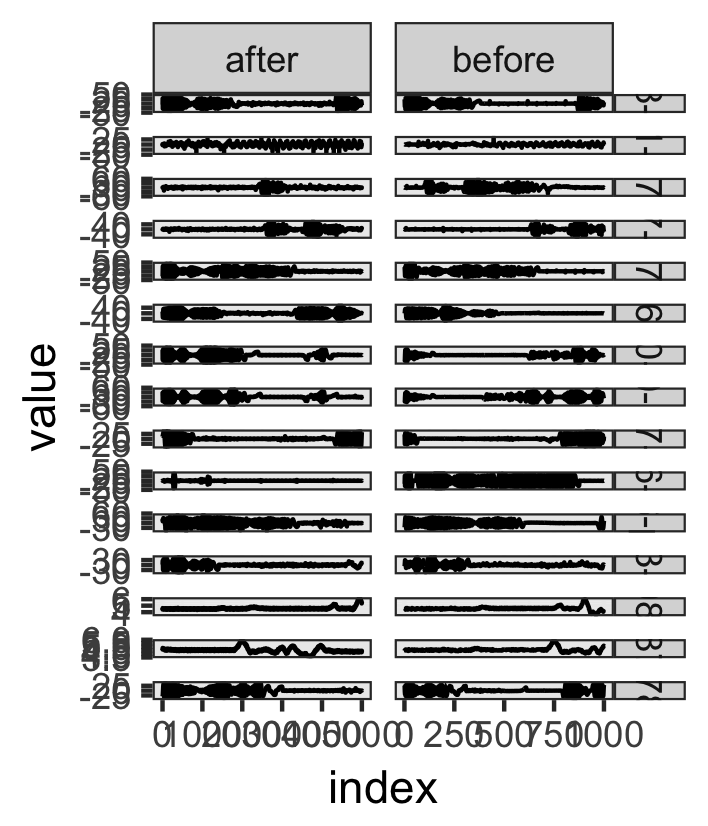
\includegraphics[width=12cm]{fig/ts.png}	
	\caption{センサーデータの時系列プロット}\label{fig:ts}
\end{center}
\end{figure}

アルファ複体のフィルトレーションを用いて$0,1,2$次元パーシステント・ホモロジーを計算した。

各次元のベッチ数を計算し、以下の図に示した

\begin{figure}[H]
\begin{center}
	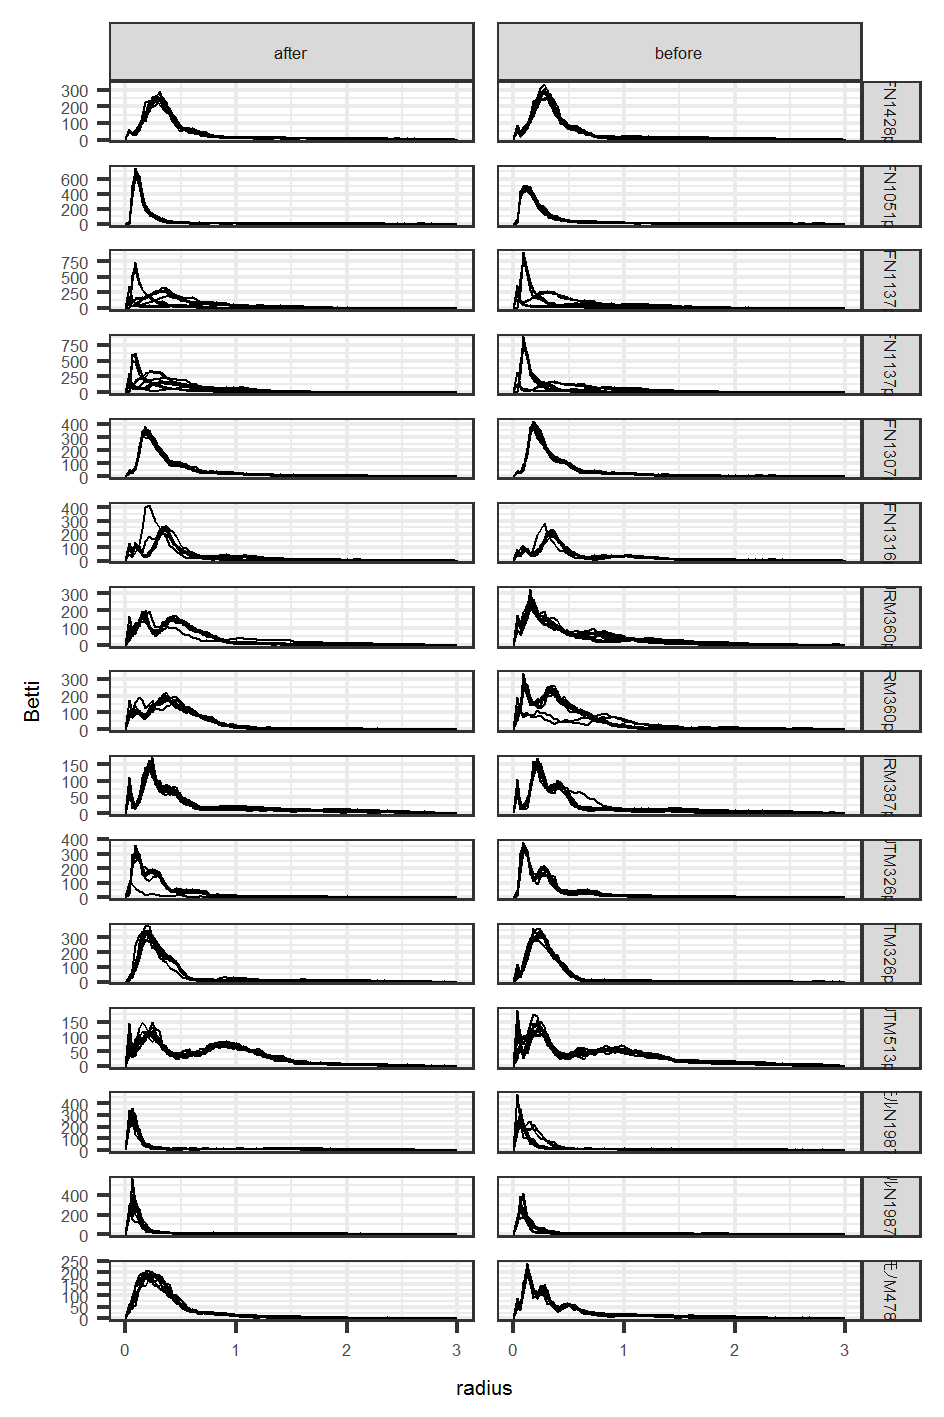
\includegraphics[width=12cm]{fig/betti_1.png}	
	\caption{1次ベッチ数}\label{fig:ts}
\end{center}
\end{figure}

\begin{figure}[H]
\begin{center}
	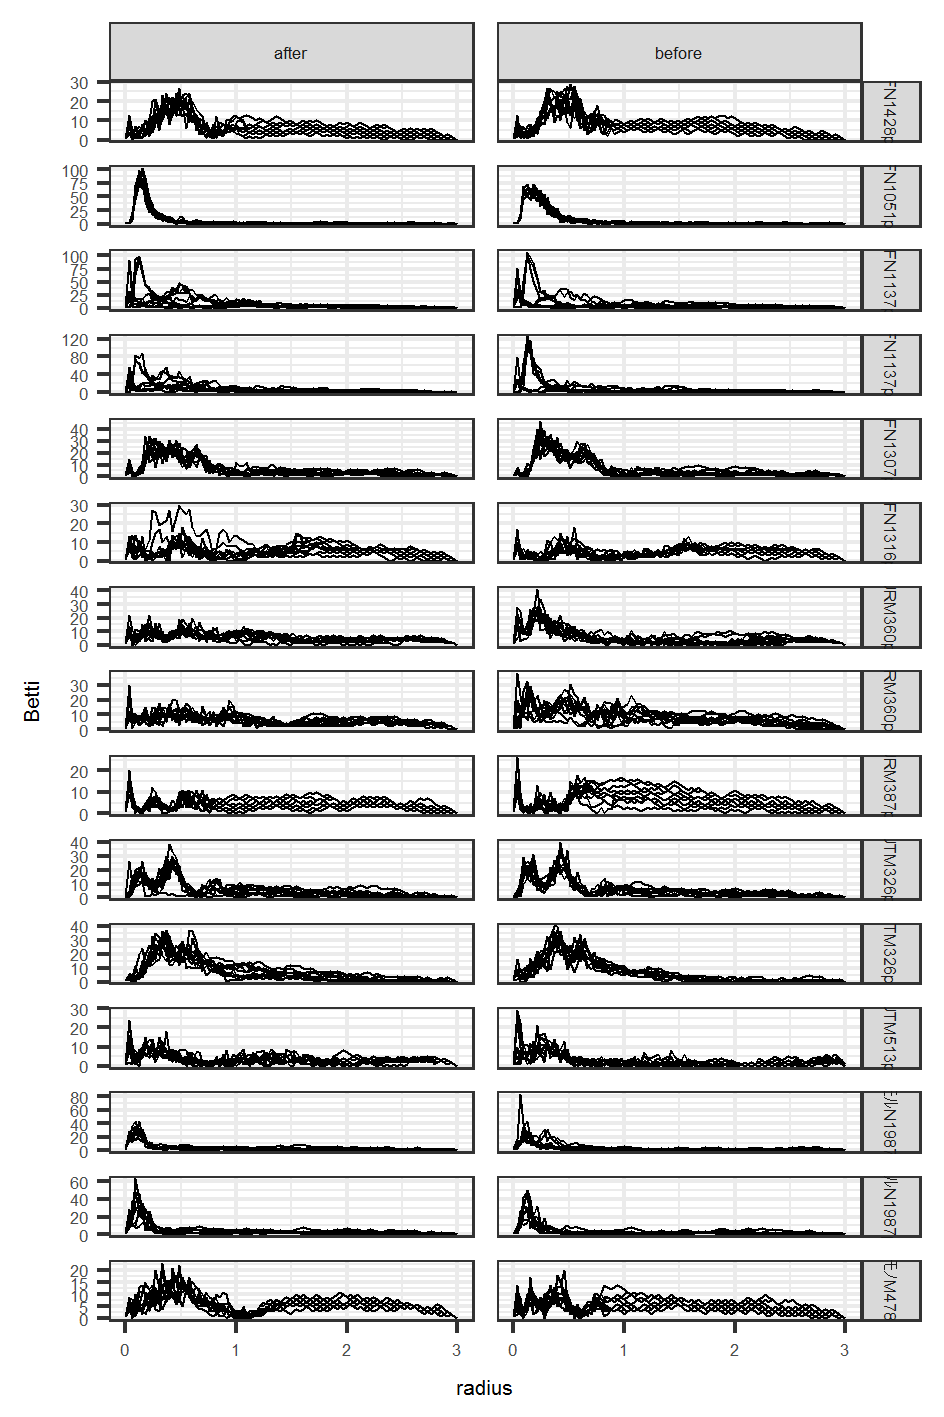
\includegraphics[width=12cm]{fig/betti_2.png}	
	\caption{2次ベッチ数}\label{fig:ts}
\end{center}
\end{figure}

ロボットアームごとに20本の系列をクラスタリングすることを考える。
1次のベッチ数をもとにDTWを比類似度とした階層的クラスタリングを行った。
クラスター間の距離は完全連結法(最遠距離法)を用いて算出した。
そのデンドログラムを以下の図\ref{fig:dendro1}から図\ref{fig:dendro15}に示した

\begin{figure}[H]
	\begin{center}
		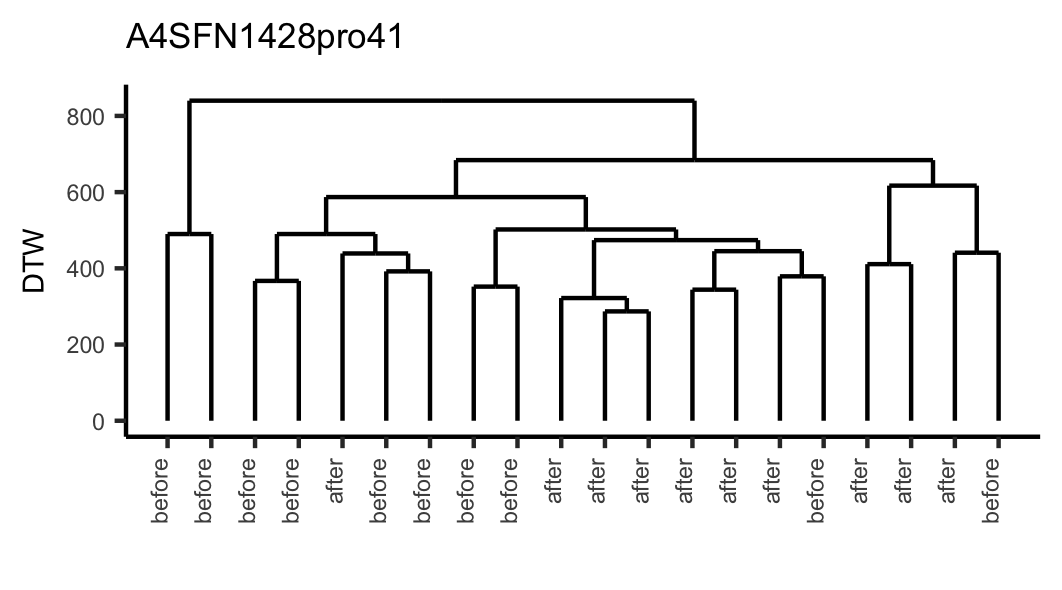
\includegraphics[width=15cm]{fig/dendro_1.png}
		\caption{デンドログラム1}
		\label{fig:dendro1}
	\end{center}
\end{figure}
\begin{figure}[H]
	\begin{center}
		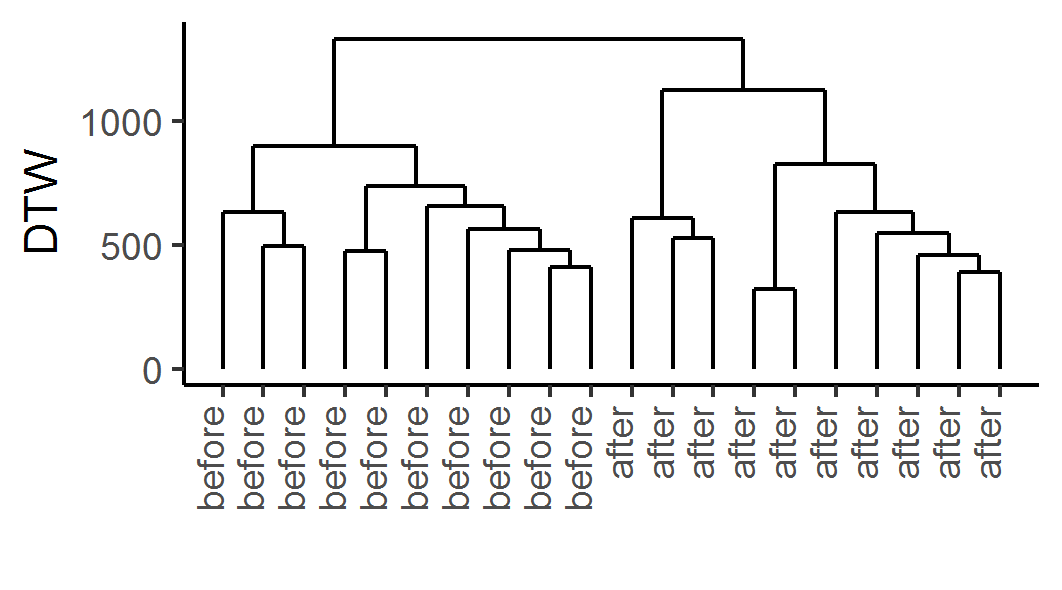
\includegraphics[width=15cm]{fig/dendro_2.png}
		\caption{デンドログラム2}
		\label{fig:dendro2}
	\end{center}
\end{figure}
\begin{figure}[H]
	\begin{center}
		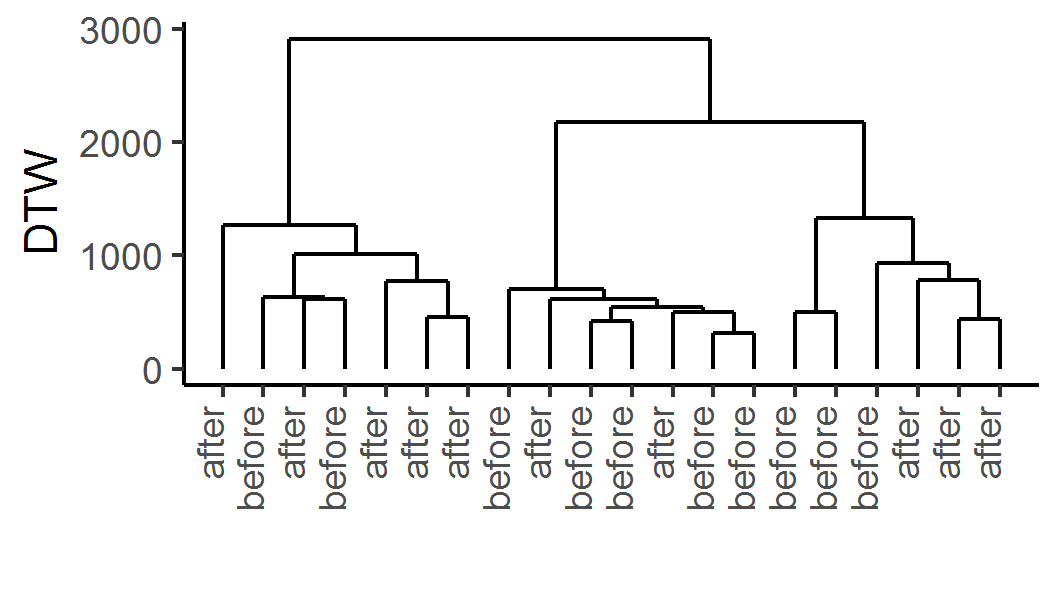
\includegraphics[width=15cm]{fig/dendro_3.png}
		\caption{デンドログラム3}
		\label{fig:dendro3}
	\end{center}
\end{figure}
\begin{figure}[H]
	\begin{center}
		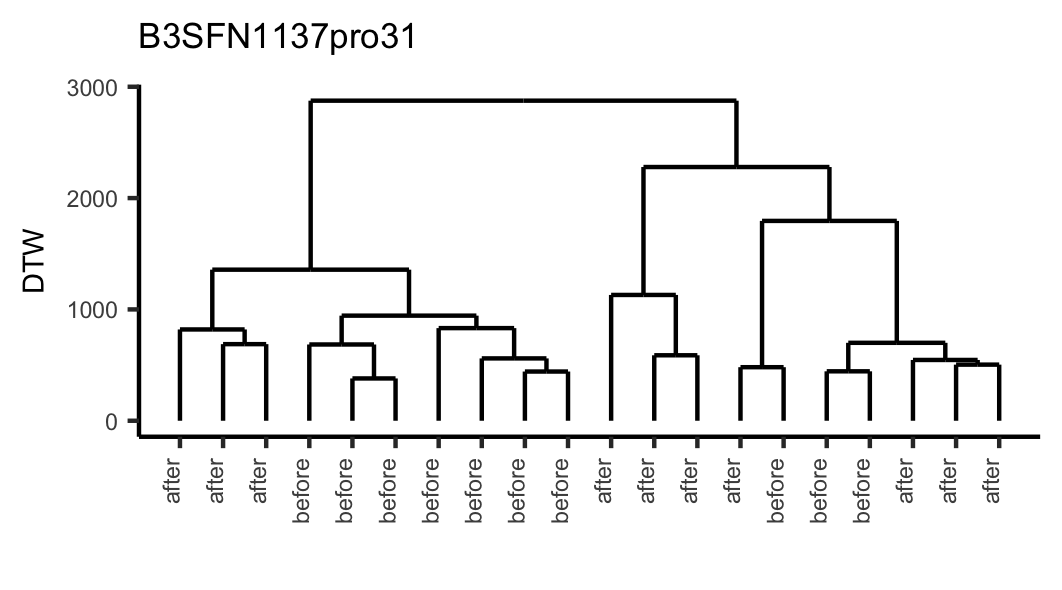
\includegraphics[width=15cm]{fig/dendro_4.png}
		\caption{デンドログラム4}
		\label{fig:dendro4}
	\end{center}
\end{figure}
\begin{figure}[H]
	\begin{center}
		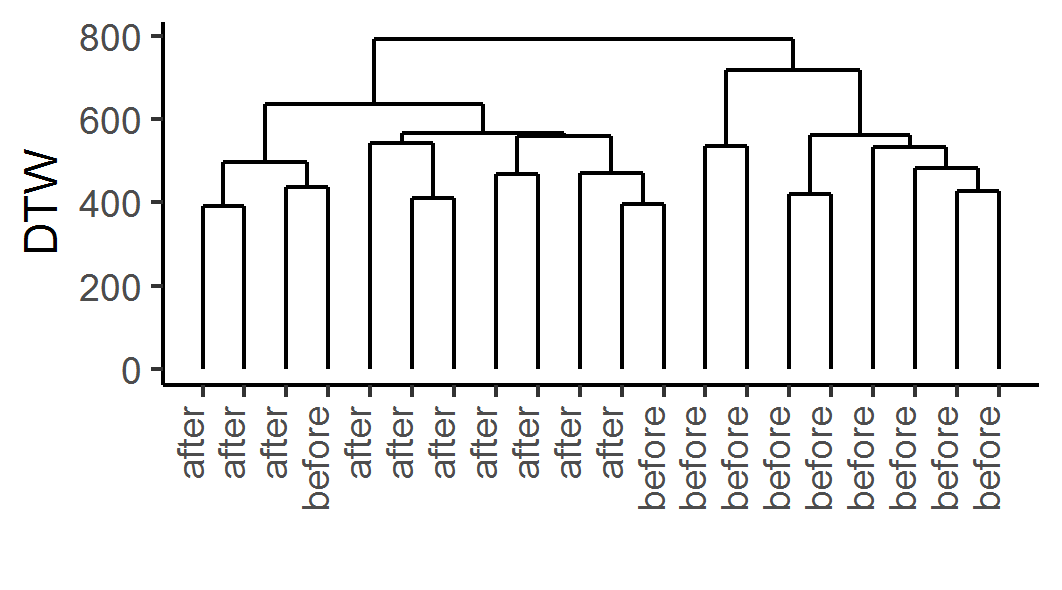
\includegraphics[width=15cm]{fig/dendro_5.png}
		\caption{デンドログラム5}
		\label{fig:dendro5}
	\end{center}
\end{figure}
\begin{figure}[H]
	\begin{center}
		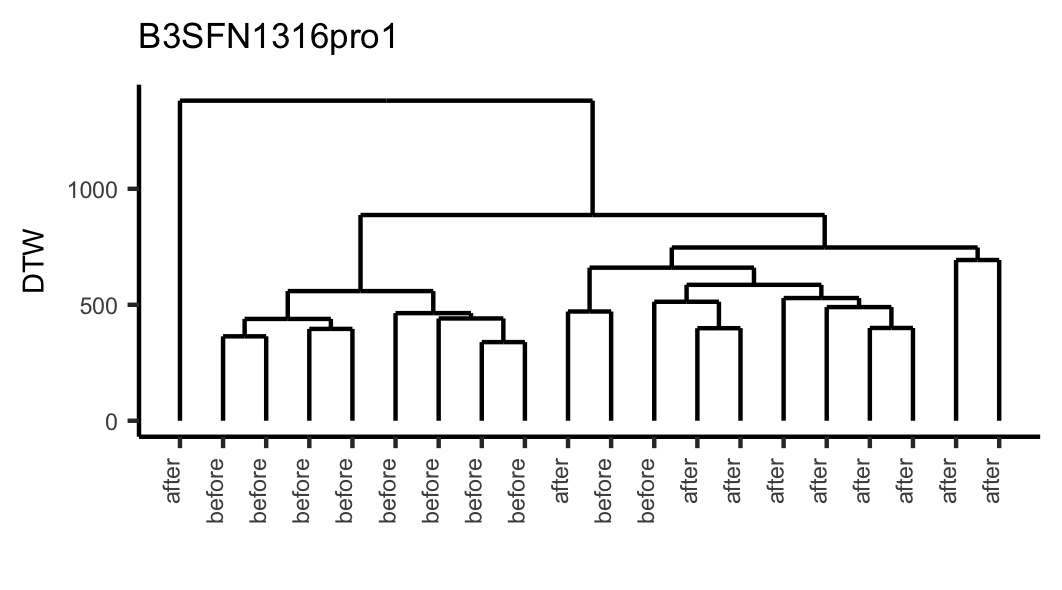
\includegraphics[width=15cm]{fig/dendro_6.png}
		\caption{デンドログラム6}
		\label{fig:dendro6}
	\end{center}
\end{figure}
\begin{figure}[H]
	\begin{center}
		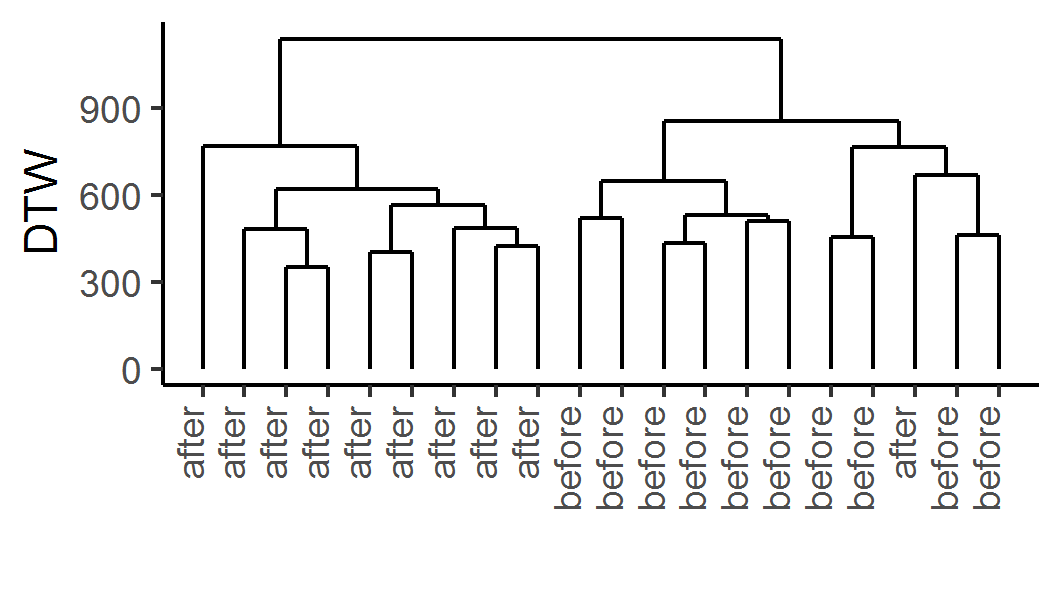
\includegraphics[width=15cm]{fig/dendro_7.png}
		\caption{デンドログラム7}
		\label{fig:dendro7}
	\end{center}
\end{figure}
\begin{figure}[H]
	\begin{center}
		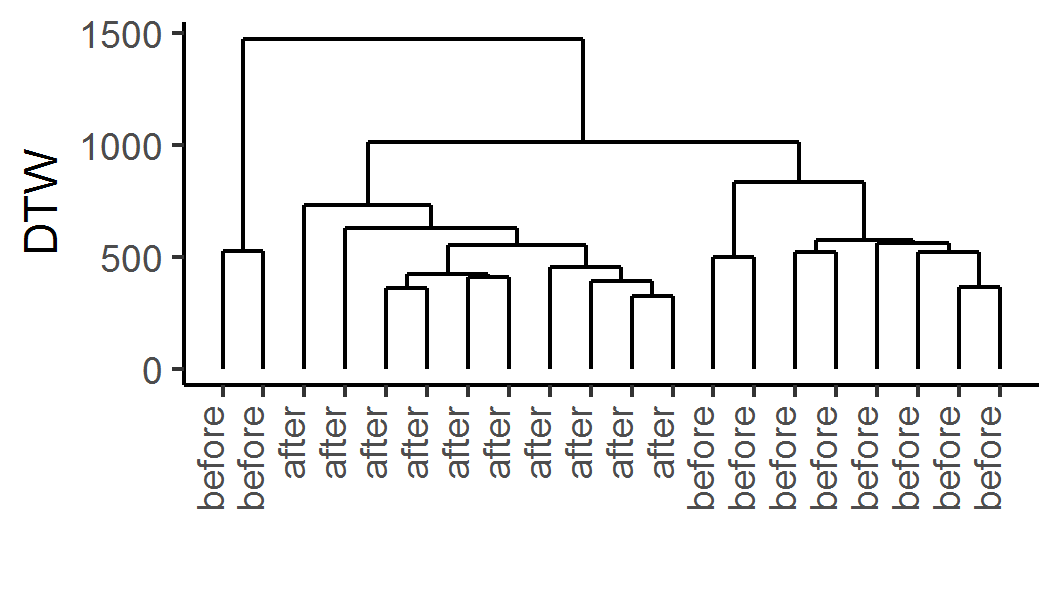
\includegraphics[width=15cm]{fig/dendro_8.png}
		\caption{デンドログラム8}
		\label{fig:dendro8}
	\end{center}
\end{figure}
\begin{figure}[H]
	\begin{center}
		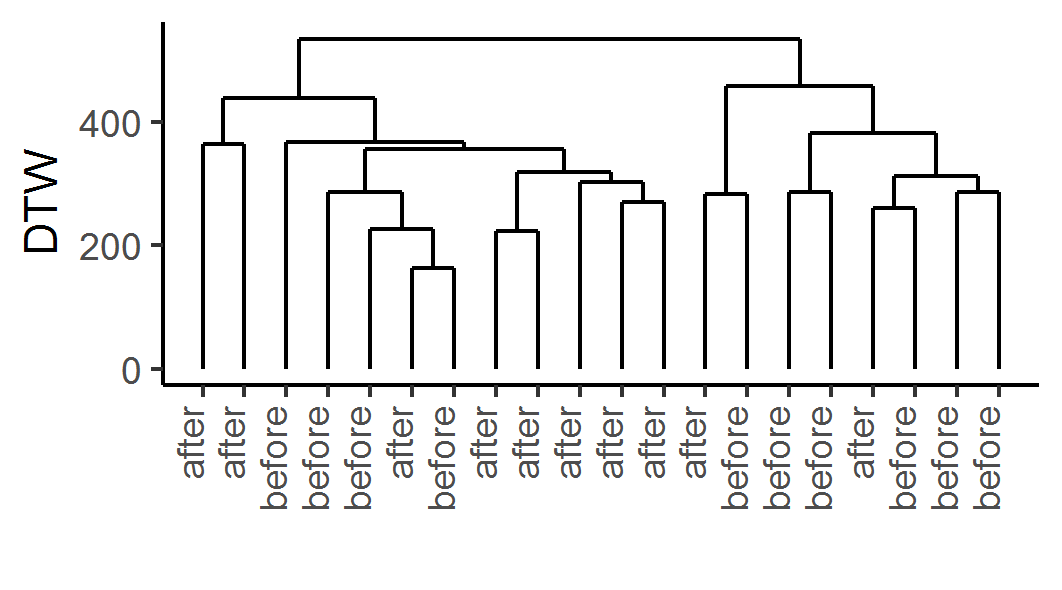
\includegraphics[width=15cm]{fig/dendro_9.png}
		\caption{デンドログラム9}
		\label{fig:dendro9}
	\end{center}
\end{figure}
\begin{figure}[H]
	\begin{center}
		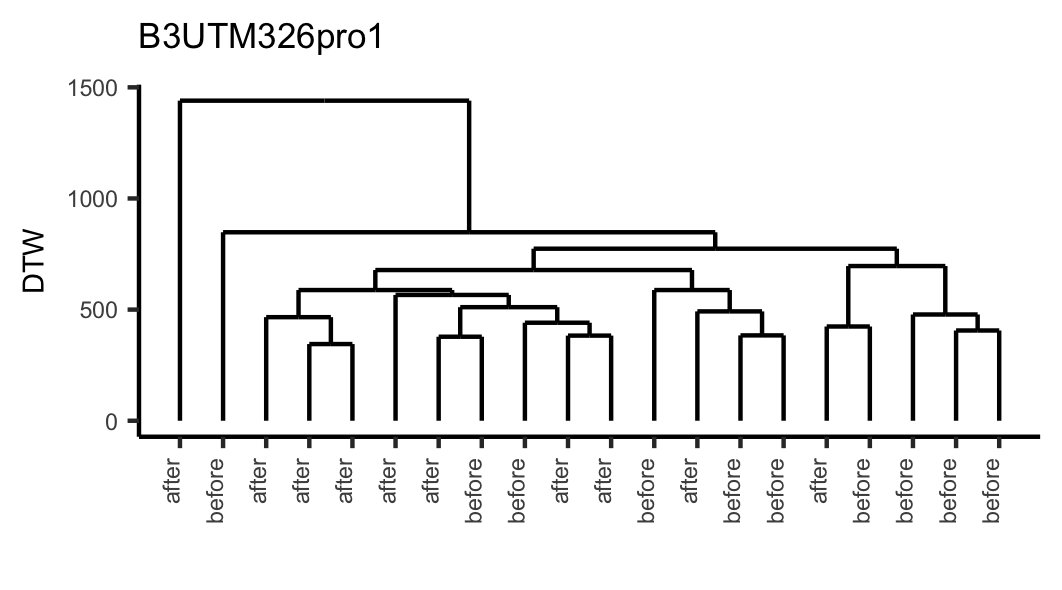
\includegraphics[width=15cm]{fig/dendro_10.png}
		\caption{デンドログラム10}
		\label{fig:dendro10}
	\end{center}
\end{figure}
\begin{figure}[H]
	\begin{center}
		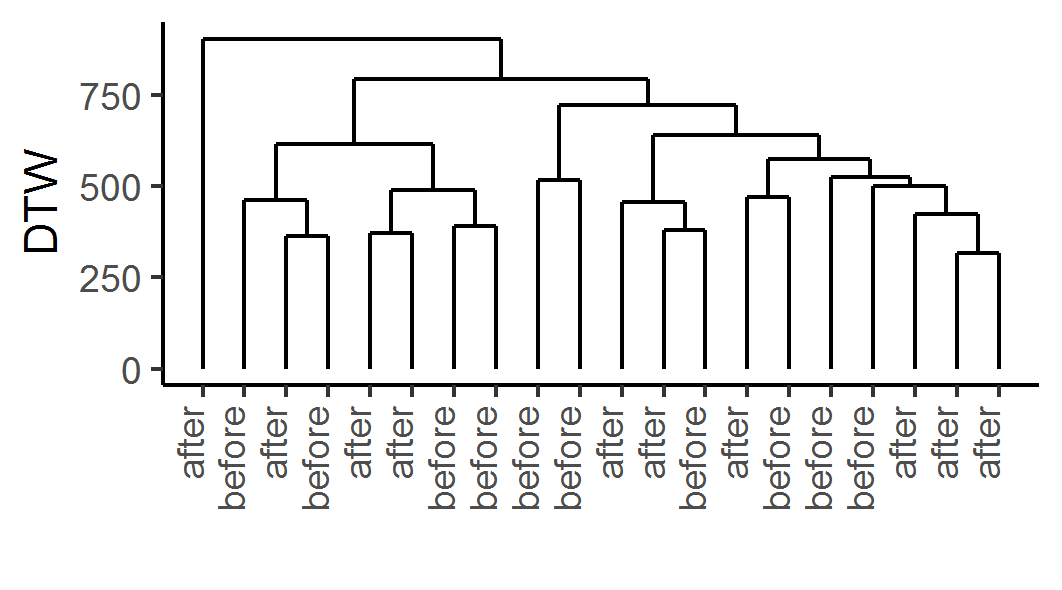
\includegraphics[width=15cm]{fig/dendro_11.png}
		\caption{デンドログラム11}
		\label{fig:dendro11}
	\end{center}
\end{figure}
\begin{figure}[H]
	\begin{center}
		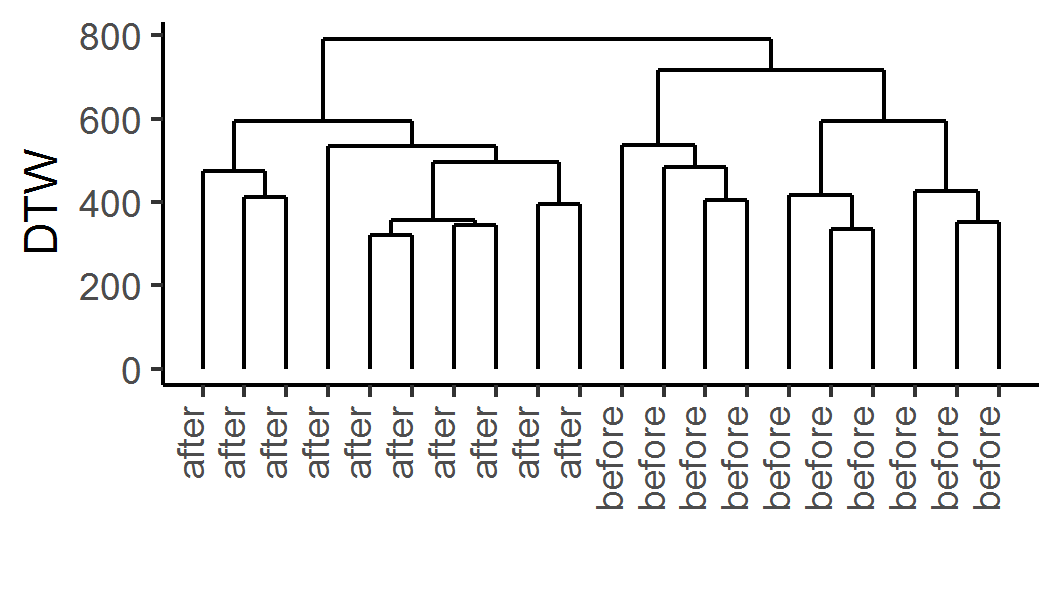
\includegraphics[width=15cm]{fig/dendro_12.png}
		\caption{デンドログラム12}
		\label{fig:dendro12}
	\end{center}
\end{figure}
\begin{figure}[H]
	\begin{center}
		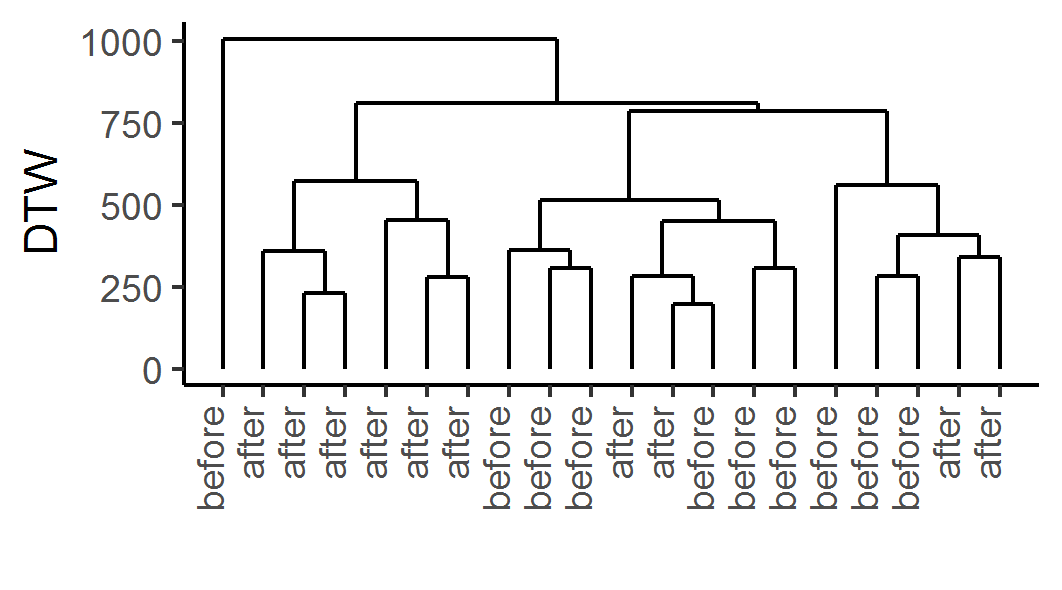
\includegraphics[width=15cm]{fig/dendro_13.png}
		\caption{デンドログラム13}
		\label{fig:dendro13}
	\end{center}
\end{figure}
\begin{figure}[H]
	\begin{center}
		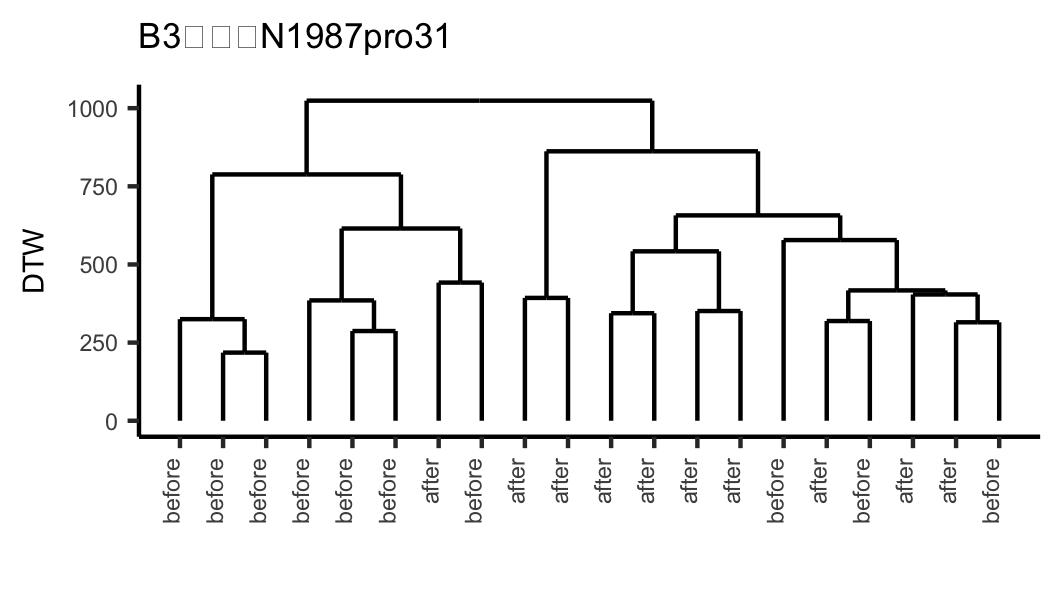
\includegraphics[width=15cm]{fig/dendro_14.png}
		\caption{デンドログラム14}
		\label{fig:dendro14}
	\end{center}
\end{figure}
\begin{figure}[H]
	\begin{center}
		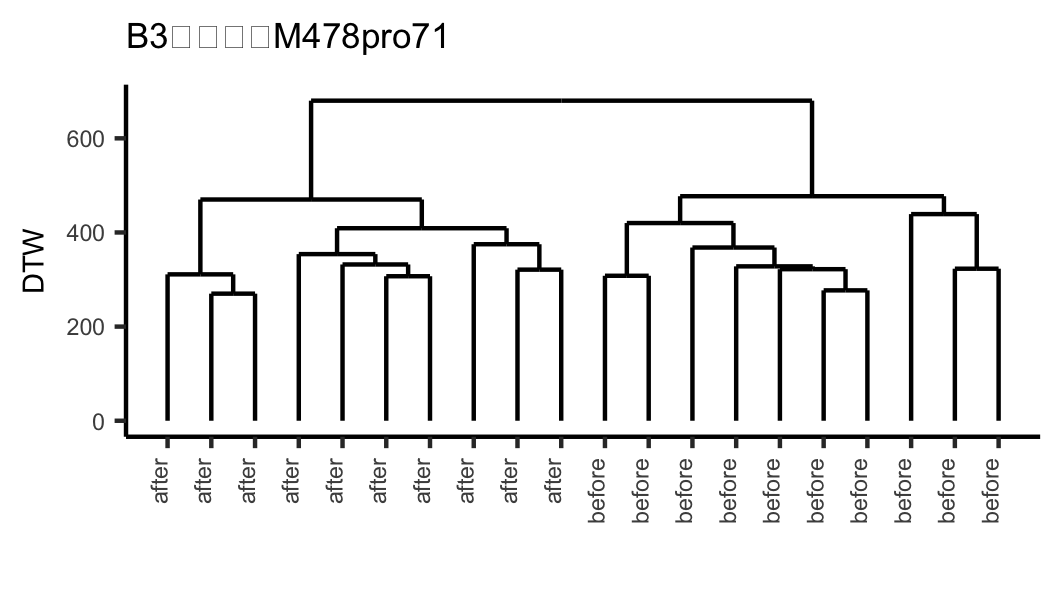
\includegraphics[width=15cm]{fig/dendro_15.png}
		\caption{デンドログラム15}
		\label{fig:dendro15}

	\end{center}
\end{figure}


\section{Persistent Diagramとその要約}


本節では,例として次の図\ref{fig:PCex}の点群を考えることとする.
\begin{figure}[H]
	\begin{center}
		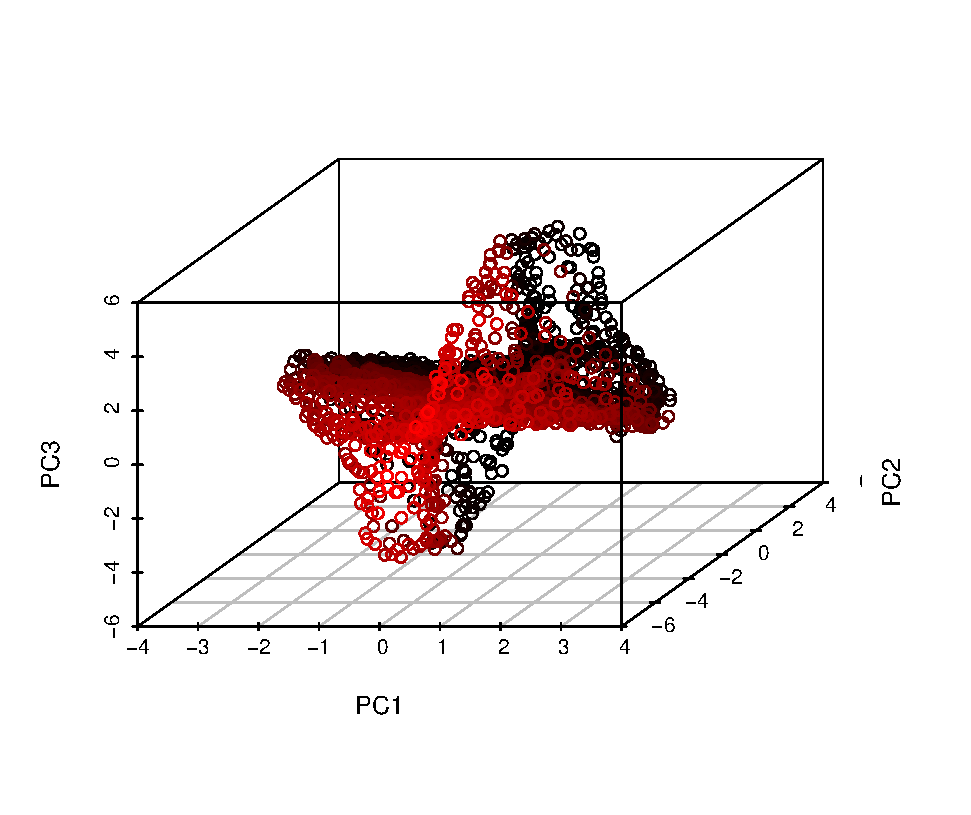
\includegraphics[width=15cm]{fig/PC_example.eps}
		\caption{Point Cloud example}
		\label{fig:PCex}
	\end{center}	
\end{figure}


\subsection{persistence diagram}
大きな情報を持つPHの直接的な表現として,Persistent Diagram(PD)と呼ばれる方法が主流である.
横軸にホモロジーが生まれる時の半径$Birth(r)$をとり,縦軸にホモロジーが消滅する時の半径$Deaty(r)$を取った散布図である.
図\ref{fig:PDex}に図\ref{fig:PCex}のPDを示した.
そのため,パーシステント・ホモロジーを要約する手法が盛んに提案されてきた.
\begin{figure}[H]
	\begin{center}
		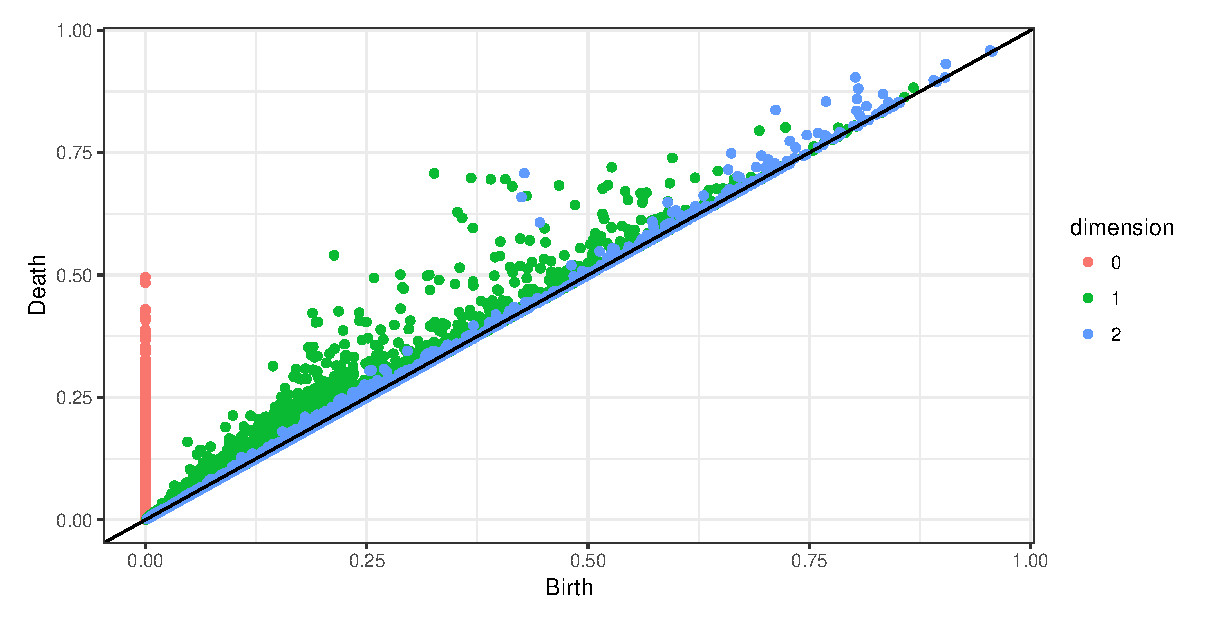
\includegraphics[width=12cm]{fig/PD_example.eps}
		\caption{Persistent Diagram example}
		\label{fig:PDex}
	\end{center}
\end{figure}
PDは散布図であるため,そこから明確な情報を読み取ることは非常に難しい.
そのため,PDを要約する手法が盛んに考えられてきた.

\subsection{maximum persistence}
PDの要約としてもっとも単純なものがmaximum persistenceである.
maximum presistenceは$i$番目の点群のpersistence diagram$D_i$の$n$次元ホモロジーに対して以下で計算され,1つの点群に由来するホモロジーに対し最大の永続性を記述する.
$$
\rm{maxPers}(D_i) = \rm{max}_{\it(birth, death)\in D_i}\it(Death(r) - Birth(r))
$$
\subsection{persistence landscape}
ノイズを含んだ実データでは,生まれてすぐに死ぬホモロジーが多数存在することになる.
つまり,より強い永続性を持ったものに着目することが重要であるとかんがえられる.
そこで,大きな永続性を持つホモロジーのみに着目する目的でpersistence landscape(PL)がしばしば用いられる.
PLは区分的な線形関数であり,$p$番目のホモロジーで$Birth(r)=b, Death(r)=d$であったとすると
\[
	\Lambda_p(t) = \begin{cases}
  	t-b, & b < t < (b+d)/2 \\
 	 d-t, & (b+d)/2< t < d\\
 	 0 & otherwise
	\end{cases}
\]

を考え,PLは
$$
F(t) = \rm{sup}\it(\Lambda_p(t))
$$
で与えられる.
図\ref{fig:PDex}PLを図\ref{fig:PLex}に示した.
\begin{figure}[H]
	\begin{center}
		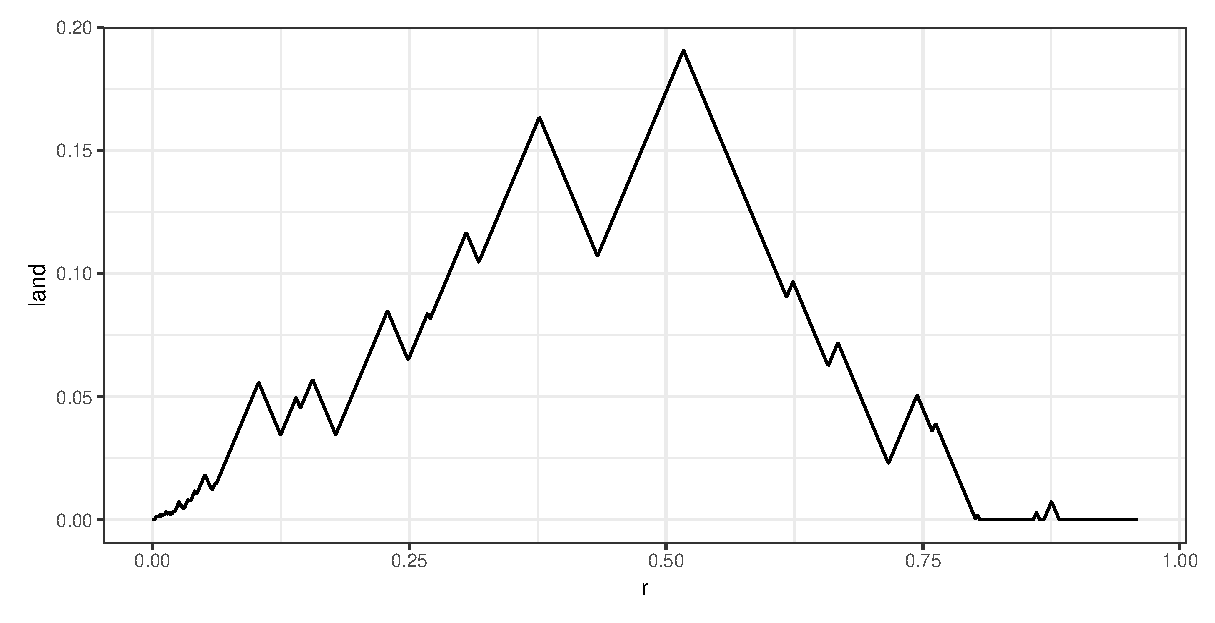
\includegraphics[width=12cm]{fig/PL_example.eps}
		\caption{Persistence Landscape example}
		\label{fig:PLex}
	\end{center}
\end{figure}

\subsection{persistence barcode}
ホモロジー$p$が生まれてから死ぬまでを実線で表して並べたものをpersistent barcodeという.
ただし,$p$の決め方に恣意性が生まれないよう注意する必要がある.
その例を図\ref{fig:PBex}に示した.左から順に0次元のホモロジー,1次元のホモロジー,2次元のホモロジーのpersistence barcodeである.
\begin{figure}[H]
	\begin{center}
		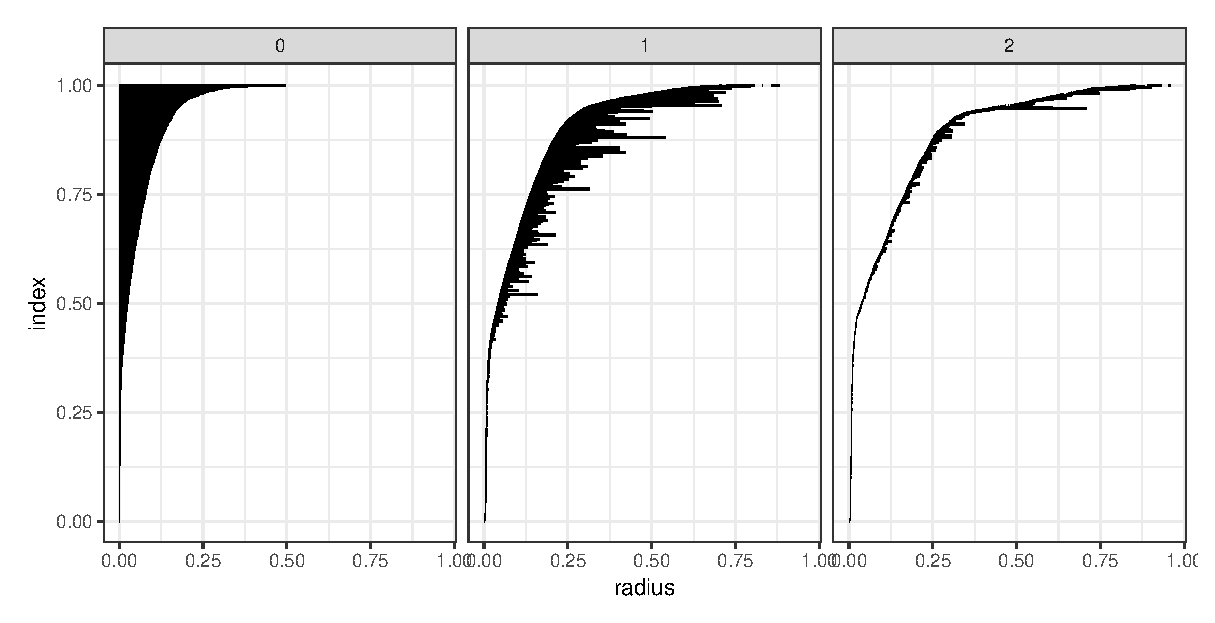
\includegraphics[width=12cm]{fig/PB_example.eps}
		\caption{Persistence Barcode example}
		\label{fig:PBex}
	\end{center}
\end{figure}


\section{時系列データに対する位相幾何学的アプローチ}
本調査で扱う時系列データは1次元のデータであるため,前節で述べたTDAのメソッドを適用するためには多次元の点群を作成する必要がある.
1次元時系列を多次元の点群に加工する手段として,時間遅れ座標を用いた埋め込みが知られている.
埋め込みは,非線形ダイナミカルシステムの分野でアトラクタを再構成するために利用される.
埋め込む次元$m$の決定にはターケンスの埋め込み定理やFFN(False Nearest Naighbors)利用することが行われている.
また,時間遅れ単位$d$は大きすぎても小さすぎてもいけないこと,明らかな周期の整数倍になってはいけないことが報告されている.

しかし,埋め込み次元$m$のを増やすとPHの計算量は指数的に増加することになる.そのため,十分多次元に埋め込んだのち,主成分分析などにより3次元に圧縮することが提案されている\cite{Truong2017}.

\section{Persistent Diagramの比較}
\subsection{Wasserstein distance}
Wasserstein distanceは,一つの変数がもう一方の(確率論的あるいは決定論的に)非一様な小さい摂動によって得られるような,二つの変数$X$と$Y$の確率分布を比較する際に自然に用いられる.
\cite{Turner2014}はPDの空間上にWasserstein distanceで距離を定義し,またその上の確率測度を調べている.



\subsection{bottleneck distance}
\cite{Bubenik2015}によって提案されたbottleneck distanceもWasserstein distanceと同様,二つのPDの類似度を測る指標である.
2つのPD(と対角線上の全ての点)が完全に一致するまでの最短距離である.
図\ref{fig:bottle}にその例を示した
\begin{figure}[H]
	\begin{center}
		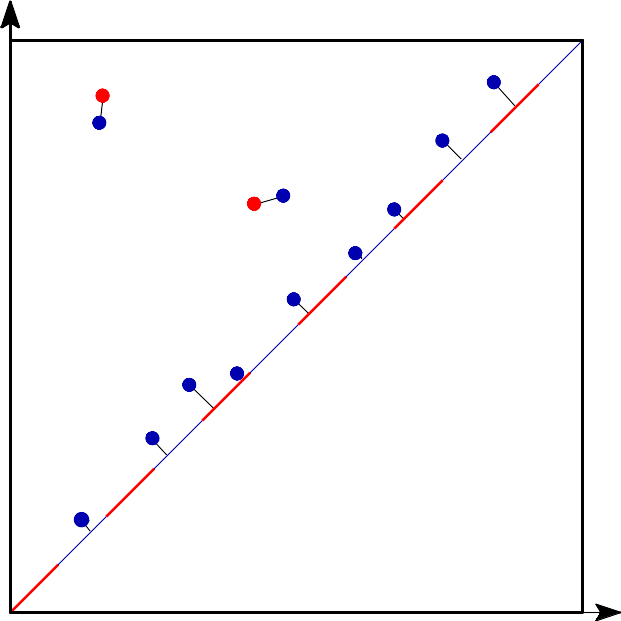
\includegraphics[width=10cm]{fig/bottleneck.png}
		\caption{bottleneck example}
		\label{fig:bottle}
	\end{center}
\end{figure}
\section{結果}

\section{考察}



\bibliography{TDA} %hoge.bibから拡張子を外した名前


\end{document}